\documentclass{llncs}
\sloppy

%%%%%%%%%%%%%%%%%%%%%%%%%%%%%%%%%%%%%%%%%%%%%%%%%%%%%%%%%%%%
% PACKAGES
%%%%%%%%%%%%%%%%%%%%%%%%%%%%%%%%%%%%%%%%%%%%%%%%%%%%%%%%%%%%
\usepackage[utf8x]{inputenc}

% SYMBOLES
\usepackage{amsmath, amssymb, url} % amsthm, 

% ALGORITHMES
\usepackage[ruled,vlined,linesnumbered]{algorithm2e}

\usepackage{subfigure}

\usepackage[pdftex,pagebackref=false,colorlinks=true]{hyperref}


%%%%%%%%%%%%%%%%%%%%%%%%%%%%%%%%%%%%%%%%%%%%%%%%%%%%%%%%%%%%
% TIKZ
%%%%%%%%%%%%%%%%%%%%%%%%%%%%%%%%%%%%%%%%%%%%%%%%%%%%%%%%%%%%
\usepackage{pgf}
\usepackage{tikz}

\graphicspath{{./figures/}}

% Couleurs
\definecolor{turquoise}{rgb}{0 0.41 0.41}
\definecolor{rouge}{rgb}{0.79 0.0 0.1}
\definecolor{vert}{rgb}{0.15 0.4 0.1}
\definecolor{mauve}{rgb}{0.6 0.4 0.8}
\definecolor{violet}{rgb}{0.58 0. 0.41}
\definecolor{orange}{rgb}{0.8 0.4 0.2}
\definecolor{bleu}{rgb}{0.39, 0.58, 0.93}
\definecolor{gris}{rgb}{0.6,0.6,0.6}
\definecolor{grisfonce}{rgb}{0.4, 0.4, 0.4}
\definecolor{grispale}{rgb}{0.9, 0.9, 0.9}
% NOIR ET BLANC
\definecolor{vertfonce}{rgb}{0.0, 0, 0.0}
\definecolor{rougefonce}{rgb}{0, 0.0, 0.0}
\definecolor{rougeclair}{rgb}{0.6, 0.6, 0.6} %{red!50!white}
\definecolor{bleufonce}{rgb}{0.2, 0.2, 0.2} %blue!80!black
\definecolor{bleutresfonce}{rgb}{0.1, 0.1, 0.1} %blue!50!black
% \definecolor{vertfonce}{rgb}{0.0, 0.5, 0.0}
% \definecolor{rougefonce}{rgb}{1, 0.0, 0.0}
% \definecolor{rougeclair}{rgb}{1, 0.5, 0.5} %{red!50!white}
% \definecolor{bleufonce}{rgb}{0, 0, 0.8} %blue!80!black
% \definecolor{bleutresfonce}{rgb}{0, 0, 0.5} %blue!50!black


% Jeu de couleurs pales
% NOIR ET BLANC
\definecolor{cpale1}{rgb}{0.6, 0.6, 0.6}
\definecolor{cpale2}{rgb}{0.9, 0.9, 0.9}
% \definecolor{cpale1}{rgb}{1, 0.6, 0.6}
% \definecolor{cpale2}{rgb}{0.6, 1, 0.6}
\definecolor{cpale3}{rgb}{0.6, 0.6, 1}
\definecolor{cpale4}{rgb}{1, 0.6, 1}
\definecolor{cpale5}{rgb}{1, 1, 0.6}
\definecolor{cpale6}{rgb}{0.6, 1, 1}
\definecolor{cpale7}{rgb}{0.95, 0.65, 0.25}
\definecolor{cpale8}{rgb}{0.75, 0.45, 1}
\definecolor{cpale9}{rgb}{0.5, 1, 0.75}
\definecolor{cpale10}{rgb}{0.8, 0.7, 0.6}
\definecolor{cpale11}{rgb}{0.6, 0.7, 0.8}
\definecolor{cpale12}{rgb}{0.2, 0.5, 0.9}
\definecolor{cpale13}{rgb}{0.5, 0.9, 0.2}
\definecolor{cpale14}{rgb}{0.9, 0.2, 0.5}
\definecolor{cpale15}{rgb}{0.7, 0.7, 0.7}
\definecolor{cpale16}{rgb}{0.8, 0.8, 0.5}



%%%%%%%%%%%%%%%%%%%%%%%%%%%%%%%%%%%%%%%%%%%%%%%%%%%%%%%%%%%%
% CONSTANTES
%%%%%%%%%%%%%%%%%%%%%%%%%%%%%%%%%%%%%%%%%%%%%%%%%%%%%%%%%%%%

%-%-%-%-%-%-%-%-%-%-%-%-%-%-%-%-%-%-%-%-%-%-%-%-%-%-%-%-%-%
% CONSTANTES MATHEMATIQUES
%-%-%-%-%-%-%-%-%-%-%-%-%-%-%-%-%-%-%-%-%-%-%-%-%-%-%-%-%-%
% Booleens
\newcommand{\false}{{\tt false}}
\newcommand{\true}{{\tt true}}

% Ensembles
\newcommand{\AP}{\mathit{AP}}
\newcommand{\grandn}{{\mathbb N}}
\newcommand{\grandq}{{\mathbb Q}}
\newcommand{\grandqplus}{{\mathbb Q}_{\geq 0}}
\newcommand{\grandr}{{\mathbb R}}
\newcommand{\grandrplus}{\grandr_{\geq 0}}
\newcommand{\grandz}{{\mathbb Z}}
\newcommand{\setX}{\mathcal{K}_{\Clock}}
\newcommand{\setP}{\mathcal{K}_{\Param}}
\newcommand{\setXP}{\mathcal{K}_{\Clock \cup \Param}}

% Matrices
\newcommand{\matrixzero}{\mathbf{0}}
\newcommand{\matrixnopath}{\emptyset}

% Noms
\newcommand{\tiling}{\mathit{Tiling}}
\newcommand{\post}{\mathit{Post}}
\newcommand{\Pre}{\mathit{Pre}}
\newcommand{\TS}{\mathit{TS}}
\newcommand{\words}{\mathit{Words}}

% Operateurs
\DeclareMathOperator*{\argmax}{arg\,max}
\DeclareMathOperator*{\argmin}{arg\,min}
\newcommand{\eqdef}{ \overset{\mathit{def}}{=}}


% Symboles
\newcommand{\cro}[1]{\langle #1 \rangle}
\newcommand{\fleche}[1]{\stackrel{#1}{\rightarrow}}
\newcommand{\Fleche}[1]{\stackrel{#1}{\Rightarrow}}
\newcommand{\prefix}[2]{ |#1|_{#2} }
\newcommand{\steps}[0]{ {\rightarrow} }
\newcommand{\Steps}[0]{ {\Rightarrow} }
\newcommand{\timelaps}[1]{#1^\uparrow}
\newcommand{\trace}[1]{ \mathbin{<}#1 \mathbin{>}}
\newcommand{\wpi}[1]{\mathbin{<}#1\mathbin{>}}

% Temporal logics
\newcommand{\tlAlways}{\Box}
\newcommand{\tlEvt}{\Diamond}
\newcommand{\tlExists}{\exists}
\newcommand{\tlForall}{\forall}
\newcommand{\tlNext}{\bigcirc} % X
% \newcommand{\tlNext}{\circle}
\newcommand{\tlUntil}{\cup}

% Unites
\newcommand{\micros}{\mathit{\mu\,s}}
\newcommand{\millis}{\mathit{m\,s}}
\newcommand{\nanos}{ns}
\newcommand{\picos}{ps}


% Variables
\newcommand{\A}{\mathcal{A}}
\newcommand{\Avar}{\A_\mathit{var}}
\newcommand{\Clock}{X} % set of clocks
\newcommand{\clock}{x} % clock
\newcommand{\clockval}{w} % clock valuation
\newcommand{\enabled}{\mathit{enabled}}
\newcommand{\events}{E} % a possible set of events
\newcommand{\EventsSet}{\Sigma} % all possible events
\newcommand{\formule}{\varphi}
\newcommand{\Formule}{\Phi}
% \newcommand{\Kinit}{K_\mathit{init}} % initial constraint on the parameters
\newcommand{\LTS}{\mathcal{L}}
\newcommand{\Param}{P} % set of parameters (P / Y)
\newcommand{\param}{p} % parameter (p / y)
\newcommand{\py}{\pi} % parameter valuation
\newcommand{\Py}{\Pi} % set of consistent parameter valuations
\newcommand{\sinit}{s_\mathit{init}} % initial set of states
\newcommand{\Slast}{S_\mathit{last}}



\newcommand{\Ko}{K_0}
\newcommand{\pio}{\pi_0}
\newcommand{\piprime}{\pi}
\newcommand{\To}{T_0}
\newcommand{\Tprime}{T}


% \newcommand{\compyes}{\textcolor{green}{yes}}
\newcommand{\compyes}{$\textcolor{vertfonce}{\mathbf{\surd}}$}
% \newcommand{\compno}{\textcolor{red}{no}}
\newcommand{\compno}{$\textcolor{rougefonce}{\mathbf{\times}}$}


% Pour MDP
\newcommand{\we}{w}
\newcommand{\We}{W}
\newcommand{\va}{v}
\newcommand{\Va}{V}
\newcommand{\prob}{\mathit{Prob}}

%-%-%-%-%-%-%-%-%-%-%-%-%-%-%-%-%-%-%-%-%-%-%-%-%-%-%-%-%-%
% PARAMETRES
%-%-%-%-%-%-%-%-%-%-%-%-%-%-%-%-%-%-%-%-%-%-%-%-%-%-%-%-%-%
% PARAMETRES BRP
\newcommand{\brpMAX}{\mathit{MAX}}
\newcommand{\brpSYNC}{\mathit{SYNC}}
\newcommand{\brpTD}{\mathit{TD}}
\newcommand{\brpTR}{\mathit{TR}}
\newcommand{\brpTun}{\mathit{T1}}

% PARAMETRES CSMACD
\newcommand{\slot}{\mathit{slot}}

% PARAMETRES FLIP FLOP
\newcommand{\THold}{T_{\mathit{Hold}}}
\newcommand{\TSetup}{T_{\mathit{Setup}}}
\newcommand{\THI}{T_{\mathit{HI}}}
\newcommand{\TLO}{T_{\mathit{LO}}}
\newcommand{\TCKQ}{T_{ \mathit{CK} \rightarrow Q}}

% PARAMETRES RCP
\newcommand{\rcpFMax}{\mathit{f\_max}} % \mathit{rc\_fast\_max}
\newcommand{\rcpFMin}{\mathit{f\_min}} % \mathit{rc\_fast\_min}
\newcommand{\rcpSMax}{\mathit{s\_max}} % \mathit{rc\_slow\_max}
\newcommand{\rcpSMin}{\mathit{s\_min}} % \mathit{rc\_slow\_min}
\newcommand{\rcpD}{\mathit{delay}}

% PARAMETRES SIMOP
\newcommand{\COMct}{\mathit{COMct}}
\newcommand{\COMd}{\mathit{COMd}}
\newcommand{\NETd}{\mathit{NETd}}
\newcommand{\PLCct}{\mathit{PLCct}}
\newcommand{\PLCmtt}{\mathit{PLCmtt}}
\newcommand{\RIOd}{\mathit{RIOd}}
\newcommand{\SIGmrt}{\mathit{SIGmrt}}

% PARAMETRES SPSMALL
\newcommand{\tSetupA}{t_\mathit{setup}^A}
\newcommand{\tSetupD}{t_\mathit{setup}^D}
\newcommand{\tSetupWen}{t_\mathit{setup}^\mathit{WEN}}


% PARAMETRES WLAN
\newcommand{\pACK}{\mathit{ACK}}
\newcommand{\pACKTO}{\mathit{ACKTO}}
\newcommand{\pASLOTTIME}{\mathit{ASLOTTIME}}
\newcommand{\pBOFF}{\mathit{BOFF}}
\newcommand{\pDIFS}{\mathit{DIFS}}
\newcommand{\pMAXCOL}{\mathit{MAXCOL}}
\newcommand{\pSIFS}{\mathit{SIFS}}
\newcommand{\pTRANSTIMEMIN}{\mathit{TTMIN}}
\newcommand{\pTRANSTIMEMAX}{\mathit{TTMAX}}
\newcommand{\pVULN}{\mathit{VULN}}


%-%-%-%-%-%-%-%-%-%-%-%-%-%-%-%-%-%-%-%-%-%-%-%-%-%-%-%-%-%
% ALGORITHMES
%-%-%-%-%-%-%-%-%-%-%-%-%-%-%-%-%-%-%-%-%-%-%-%-%-%-%-%-%-%
% Algorithmes PTA
\newcommand{\IM}{\mathit{IM}}
\newcommand{\IMincl}{\IM_\subseteq}
\newcommand{\IMK}{\IM^K}
\newcommand{\IMunion}{\IM^\cup}
\newcommand{\IMinclK}{\IM^K_\subseteq}
\newcommand{\IMinclunion}{\IM^\cup_\subseteq}
\newcommand{\IMotf}{\IM_\mathit{otf}}
\newcommand{\BC}{\mathit{BC}}
\newcommand{\BCincl}{\BC_\subseteq}
\newcommand{\BCK}{\BC^K}
\newcommand{\BCunion}{\BC^\cup}
\newcommand{\BCinclK}{\BC^K_\subseteq}
\newcommand{\BCinclunion}{\BC^\cup_\subseteq}


%-%-%-%-%-%-%-%-%-%-%-%-%-%-%-%-%-%-%-%-%-%-%-%-%-%-%-%-%-%
% CONSTANTES DE CHAINES
%-%-%-%-%-%-%-%-%-%-%-%-%-%-%-%-%-%-%-%-%-%-%-%-%-%-%-%-%-%

% Langue
\newcommand{\absurde}{\emph{reductio ad absurdum}}

% Divers (projets et technique)

\newcommand{\lipsix}{LIP\,6}
\newcommand{\parissix}{Universit\'e Pierre et Marie Curie}
\newcommand{\simop}{SIMOP}
\newcommand{\spsmall}{SPSMALL}
\newcommand{\stm}{ST-Microelectronics}
\newcommand{\therac}{Therac-25}
\newcommand{\valmem}{VALMEM}

% Outils
\newcommand{\apron}{\textsc{Apron}}
\newcommand{\gdot}{\textsc{dot}}
\newcommand{\graphviz}{Graphviz}
\newcommand{\hytech}{{\sc HyTech}}
\newcommand{\imitator}{\textsc{Imitator}}
% \newcommand{\imitatordeux}{\textsc{Imitator}\,II}
\newcommand{\hymitator}{\textsc{Hymitator}}
\newcommand{\kronos}{\textsc{Kronos}}
\newcommand{\nusmv}{NuSMV}
\newcommand{\ocaml}{OCaml}
\newcommand{\phaver}{PHAVer}
\newcommand{\plot}{gnuplot}
\newcommand{\polka}{NewPolka}
\newcommand{\prism}{\textsc{Prism}}
\newcommand{\python}{Python}
\newcommand{\red}{RED}
\newcommand{\romeo}{Rom\'eo}
\newcommand{\smv}{SMV}
\newcommand{\spin}{Spin}
\newcommand{\tina}{TINA}
\newcommand{\trex}{\textsc{TReX}}
\newcommand{\uppaal}{\textsc{Uppaal}}
\newcommand{\vhdlta}{\textsc{Vhdl2Ta}}






%%%%%%%%%%%%%%%%%%%%%%%%%%%%%%%%%%%%%%%%%%%%%%%%%%%%%%%%%%%%
% FORMATING
%%%%%%%%%%%%%%%%%%%%%%%%%%%%%%%%%%%%%%%%%%%%%%%%%%%%%%%%%%%%

% CODE INTEGRE AU TEXTE
\newcommand{\code}[1]{\textbf{\texttt{#1}}}

% COMMENTAIRE DANS UN ALGORITHME
\newcommand{\comalgo}[1]{\textcolor{grisfonce}{\tcp*{ #1 }}}


% COMMENTAIRES DANS UN PARAGRAPHE
% \newcommand{\commentaire}[1]{\textcolor{red}{\textbf{$\Leftarrow$  #1 $\Rightarrow$}}}
\newcommand{\commentaire}[1]{}

% REDEFINITIONS DES PARAGRAPHES
\newcommand{\paragraphe}[1]{\paragraph{#1.}}
% \newcommand{\paragraphe}[1]{\subsubsection{#1.}}

\renewcommand{\baselinestretch}{0.98}
\addtolength{\textheight}{0.2cm}

% Title
% \title{Efficient Analysis of Parametric Hybrid Systems with HYMITATOR}
\title{Parametric Analysis of Hybrid Systems Using HYMITATOR}
% \thanks{A long version of this paper is available in~\cite{AS11}, with full preliminary definitions, and all detaild algorithms and proofs.}
\author{\'Etienne Andr\'e$^1$ and %Laurent Fribourg$^2$,
	Ulrich K\"uhne$^2$% and Romain Soulat$^2$
	}
\institute{$^1$LIPN, CNRS UMR 7030, Université Paris 13, France \\
% $^2$ENS Cachan, CNRS, LSV, UMR8643 \\
$^2$Group for Computer Architecture, University of Bremen, Germany}


\begin{document}

\maketitle

\begin{abstract}
	Hybrid automata are a powerful formalism for modeling and verifying hybrid systems, that combine continuous and discrete behavior.
	A common problem in hybrid system verification is the good parameters problem, which consists in identifying a set of parameter valuations which guarantee a certain behavior of a system.
	We introduce here \hymitator{}, a tool allowing efficient parameter synthesis for hybrid automata, and providing the system with a quantitative measure of its robustness.
\end{abstract}

\keywords{Hybrid automata, Verification, Parameter synthesis, Robustness}

\commentaire{Version avec commentaires}


%%%%%%%%%%%%%%%%%%%%%%%%%%%%%%%%%%%%%%%%%%%%%%%%%%%%%%%%%%%%
%%%%%%%%%%%%%%%%%%%%%%%%%%%%%%%%%%%%%%%%%%%%%%%%%%%%%%%%%%%%
\section{Motivation and History}
%%%%%%%%%%%%%%%%%%%%%%%%%%%%%%%%%%%%%%%%%%%%%%%%%%%%%%%%%%%%
%%%%%%%%%%%%%%%%%%%%%%%%%%%%%%%%%%%%%%%%%%%%%%%%%%%%%%%%%%%%

%% \commentaire{short introduction}

Hybrid systems combine discrete and continuous behavior.
This corresponds for instance to the discrete control logic and continuous physical variables in an embedded system.
Hybrid automata are a popular and powerful model for such systems, where the continuous variables evolve according to ordinary differential equations in each control mode.

In~\cite{acef09}, we proposed the \emph{inverse method} for timed automata, a subclass of hybrid systems whose variables (named clocks) all have constant rates equal to~1.
Different from CEGAR-based methods, this original semi-algorithm for parameter synthesis is based on a ``good'' parameter valuation (also named \emph{point})~$\pio$ instead of a set of ``bad'' states.
This method synthesizes a constraint~$\Ko$ on the parameters such that, for each parameter valuation~$\piprime$ satisfying $\Ko$, the trace set (i.e., the discrete behavior) of~$\A$ under~$\piprime$ is the same as for~$\A$ under~$\pio$.
This preserves in particular linear time properties.
This also provides the system with a criterion of robustness, in the sense that the resulting constraint gives a quantitative measure of the allowed ``drift'' such that the discrete behavior of the system is not impacted.
By iterating the inverse method on all integer points within a bounded reference parameter domain, we get a set of constraints (or \emph{tiles}) such that, for each parameter valuation in each such tile, the time-abstract behavior is the same: this gives a \emph{behavioral cartography} of the system~\cite{af10}.

A basic implementation named \imitator{} (for \emph{Inverse Method for Inferring Time AbstracT behaviOR}) has first been proposed%in~\cite{and09}
, under the form of a \python{} script calling \hytech{}.
The tool has then been entirely rewritten in \imitator{}\,2.0~\cite{and10}, under the form of a standalone \ocaml{} program making use of the Parma Polyhedra Library (PPL)~\cite{bhz08}.
A number of case studies containing up to 60 timing parameters could be efficiently verified in the purely timed framework.
The latest version (2.5) includes stopwatches and arbitrary updates, and has been applied to several classes of scheduling problems~\cite{afks}.

The inverse method and the behavioral cartography have been extended to hybrid systems in~\cite{FK11}.
Due to the strong syntactic and algorithmic differences between timed automata and hybrid automata, the work of~\cite{FK11} had to be implemented in an experimental ``fork'' of \imitator{}\,2.0, and not in the main version.
% \commentaire{small description to add}
We present in this paper \hymitator{}, a now mature extension of that prototype, performing parameter synthesis on hybrid systems.

% It would be unfortunately hard (if not impossible) to merge \imitator{} with \hymitator{}; the 




% 
% 
% \commentaire{Laurent a dit :}
% - le principe de la methode inverse pour les TA a été implémenté de façon basique ([ICTAC09])
% puis de façon sophistiquée ([Infinity10])
% 
% - la méthode a été étendue pour les HA et implémentée de façon basique ([RP11])
% 
% - il s'agit "ici" de décrire une implémentation sophistiquée (intégrant notamment des extensions
% du merging des TA  à la  [NFM 12] aux HA)
% 

%%%%%%%%%%%%%%%%%%%%%%%%%%%%%%%%%%%%%%%%%%%%%%%%%%%%%%%%%%%%
%%%%%%%%%%%%%%%%%%%%%%%%%%%%%%%%%%%%%%%%%%%%%%%%%%%%%%%%%%%%
\section{Implementation and Features}
%%%%%%%%%%%%%%%%%%%%%%%%%%%%%%%%%%%%%%%%%%%%%%%%%%%%%%%%%%%%
%%%%%%%%%%%%%%%%%%%%%%%%%%%%%%%%%%%%%%%%%%%%%%%%%%%%%%%%%%%%

\hymitator{} takes as input a network of hybrid automata synchronized on shared actions.
The input syntax, inspired by \hytech{}% and \imitator{}
, allows the use of analog variables (such as time, velocity or temperature), rational-valued discrete variables, and parameters (i.e., unknown constants). The dynamics of the analog variables is described by ordinary differential equations. The tool directly supports linear dynamics, while affine dynamics can be approximated with arbitrary precision.

The core of the program is written in the object-oriented language OCaml, and interacts with~PPL.
Exact arithmetics with unbounded precision is used.
A constraint is output in text format; furthermore, the set of traces computed by the analysis can be output under a graphical form (using \graphviz{}).

% %-%-%-%-%-%-%-%-%-%-%-%-%-%-%-%-%-%-%-%-%-%-%-%-%-%-%-%-%-%-%
% \begin{figure}[ht!]
% 	% STYLES
% 	\tikzstyle{etiquette} = [draw=none, color=black]
% 	
% % \tikzstyle{boite}=[text width=8em, text centered, minimum height=2.5em, rounded corners, very thick]
% % \tikzstyle{input}=[boite, draw=green!20!gris, top color=green!50, bottom color=green!10!white]
% % \tikzstyle{output}=[boite, draw=red!20!gris, top color=red!50, bottom color=red!5!white]
% % \tikzstyle{imitator} = [boite, draw=blue!20!gris, text width=10em, minimum height=6em]
% 
% 	
% 	\tikzstyle{boite}=[rectangle, draw=black, rounded corners, thick, draw=blue!40!black, top color=blue!20, bottom color=blue!5!white]
% % 	\tikzstyle{imitator} = [boite]
% % 	\tikzstyle{apron} = [boite, draw=yellow!20!gris, top color=yellow!70, bottom color=yellow!10!white]
% % 	\tikzstyle{polka} = [apron]
% % 	\tikzstyle{ppl} = [apron]
% 	\tikzstyle{dot} = [boite, draw=purple!20!gris, top color=purple!60, bottom color=purple!10!white]
% 
% 	\tikzstyle{fleche} = [->, draw=black, semithick]
% {
% 
% \centering
% 
% \begin{tikzpicture}[scale=0.6,  =>stealth']
% 
% 	% Boites
% 	\draw[boite] (-5, 5.5) rectangle (-2, 6.5);
% 	\node [etiquette] at (-3.5, 6) {Model};
% 	
% 	\draw[boite] (-5, 3.8) rectangle (-2, 5);
% 	\node [etiquette] at (-3.5, 4.4) {\begin{tabular}{c}Reference\\valuation\end{tabular}};
% 	
% 	\draw[boite] (0, 4) rectangle (6, 6.5);
% 	\node [etiquette] at (3, 5.25) {\large \hymitator{}};
% 	
% 	\draw[boite] (1, 2.5) rectangle (5, 3.5);
% 	\node [etiquette] at (3, 3) {PPL};
% 	
% 	\draw[boite] (8, 5.5) rectangle (12, 6.5);
% 	\node [etiquette] at (10, 6) {Constraint};
% 	
% 	\draw[boite] (8, 4) rectangle (12, 5);
% 	\node [etiquette] at (10, 4.5) {Trace set};
% 
% 	% Fleches
% 	\path[fleche] (-2, 6) --++ (2, 0);
% 	\path[fleche] (-2, 4.4) --++ (2, 0);
% 	\path[fleche] (3.5, 4) --++ (0, -.5);
% 	\path[fleche] (2.5, 3.5) --++ (0, .5);
% 	\path[fleche] (6, 6) --++ (2, 0);
% 	\path[fleche] (6, 4.5) --++ (2, 0);
% 
% \end{tikzpicture}
% 
% }
% 
% \caption{Architecture of \hymitator{}}
% \label{fig:structure}
% \end{figure}
% %-%-%-%-%-%-%-%-%-%-%-%-%-%-%-%-%-%-%-%-%-%-%-%-%-%-%-%-%-%-%

\hymitator{} implements the following algorithms for hybrid systems:
\begin{description}
	\item[Full reachability analysis] Given a model, it computes the set of symbolic reachable states.
\item[Predicate Abstraction] Safety verification can alternatively be performed using a counterexample-guided abstraction refinement loop. The abstract state space is constructed w.r.t.~a set of linear predicates%. The method has been described in
	~\cite{ADI2006}.
	\item[Inverse method] Given a model and a reference parameter valuation~$\pio$, it computes a constraint on the parameter guaranteeing the same time-abstract behavior as under~$\pio$~\cite{acef09,FK11}.
	\item[Behavioral cartography] Given a model and a bounded parameter domain for each parameter valuation, it computes a set of constraints~\cite{af10,FK11}.% and their corresponding trace sets.
\end{description}

\hymitator{} uses several algorithmic optimizations, some of which have initially been developed for \imitator{}.
In particular, the efficient merging technique presented in~\cite{AFS12} has been successfully extended to the hybrid case: we merge any two states sharing the same discrete part (location and value of the discrete variables) and such that the union of their constraint on the analog variables and parameters is convex.
This optimization preserves the correctness of all our algorithms; better, the constraint output by the inverse method in that case may be weaker, i.e., covers a larger set of parameter valuations.

For affine hybrid systems, further optimizations are needed. Due to the linear over-approximation by partitioning the state space, a lot of additional branching is introduced, which renders the inverse method ineffective. To solve this problem, the algorithm has been extended as described in~\cite{FK11}. Basically, the partitioning is performed locally, and partitions belonging to the same discrete state are merged by taking their convex hull. 

The post image computation can be costly for hybrid automata. To overcome this problem, an abstraction technique for the verification of simple safety  properties (non-reachability of bad states) has been presented in~\cite{ADI2006}. Based on a set of linear predicates, reachability is performed on the abstract state space induced by these predicates. Refinement can be performed by discovering separation planes. While the original method is based on flow-pipe construction, we adapted the algorithm to the linear approximation by state space partitioning. 

%% \commentaire{un mot sur la cartographie puisque, je crois, elle a ete modifiee dans le cas des systemes hybrides}

The behavioral cartography has been adapted to the framework of hybrid systems.
Different  from timed automata, hybrid automata do not restrict coefficients appearing in clock constraints to be integers, and allow variables to be compared with any rational value.
For this reason, instead of considering only integer points as starting points for the inverse method, an arbitrary rational step size can be used for each parameter dimension in \hymitator{}.
This gives more accurate results, by reducing the size of the possible ``holes'' not covered by any tile of the cartography.

\hymitator{} (with sources, binaries and case studies) is available on its Web page: \url{http://www.lsv.ens-cachan.fr/Software/hymitator/}.



%%%%%%%%%%%%%%%%%%%%%%%%%%%%%%%%%%%%%%%%%%%%%%%%%%%%%%%%%%%%
%%%%%%%%%%%%%%%%%%%%%%%%%%%%%%%%%%%%%%%%%%%%%%%%%%%%%%%%%%%%
\section{Applications}
%%%%%%%%%%%%%%%%%%%%%%%%%%%%%%%%%%%%%%%%%%%%%%%%%%%%%%%%%%%%
%%%%%%%%%%%%%%%%%%%%%%%%%%%%%%%%%%%%%%%%%%%%%%%%%%%%%%%%%%%%


%-%-%-%-%-%-%-%-%-%-%-%-%-%-%-%-%-%-%-%-%-%-%-%-%-%-%-%-%-%-%
\begin{figure}[t]
	\centering
	\subfigure[Reachable states]{
		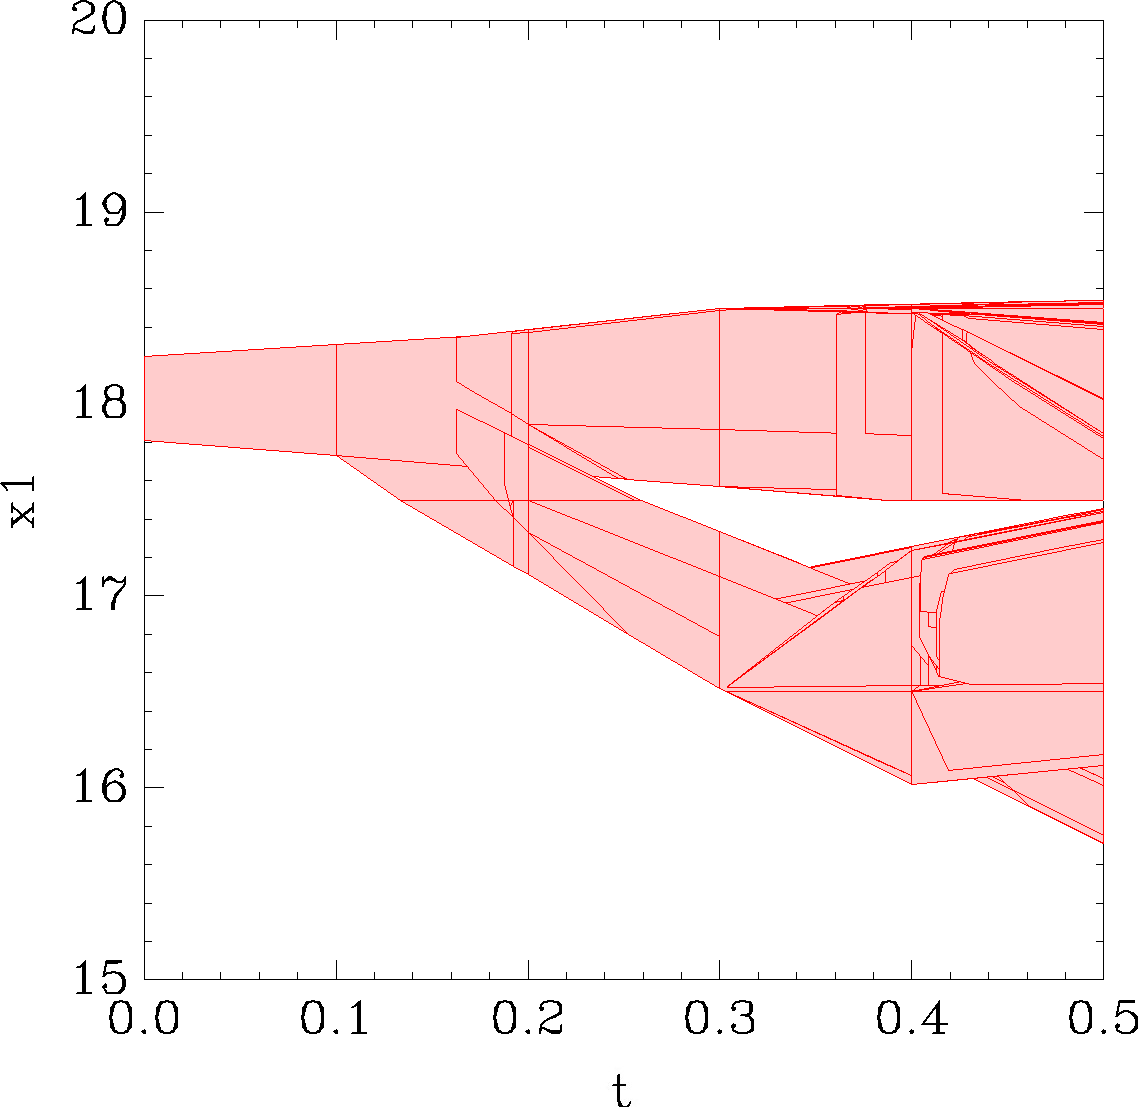
\includegraphics[width=3.6cm]{plot_t_x1}
		\label{fig:plot1}
	}
%     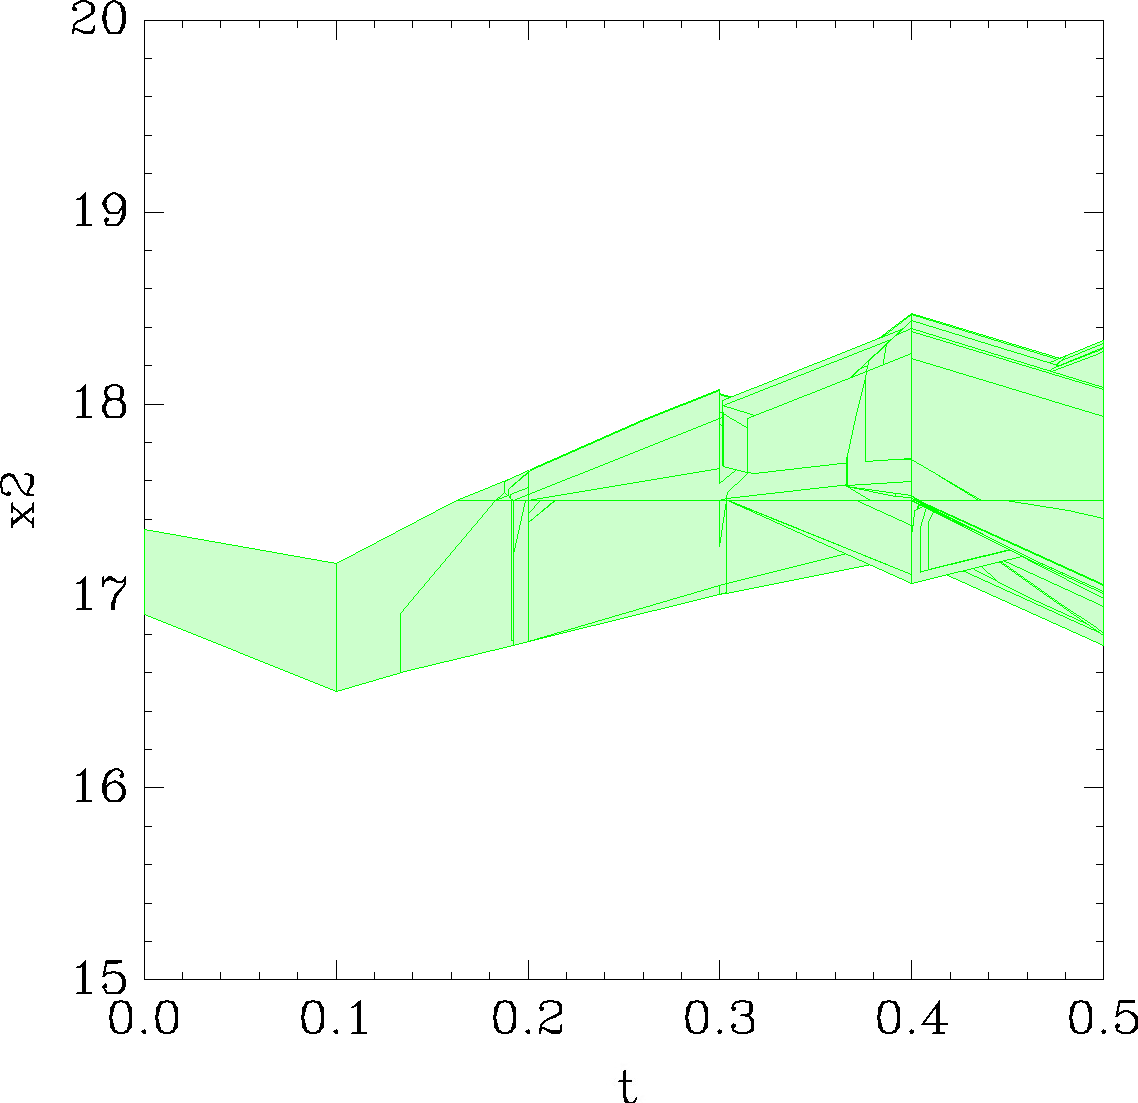
\includegraphics[width=3.5cm]{plot_t_x2} \;
%     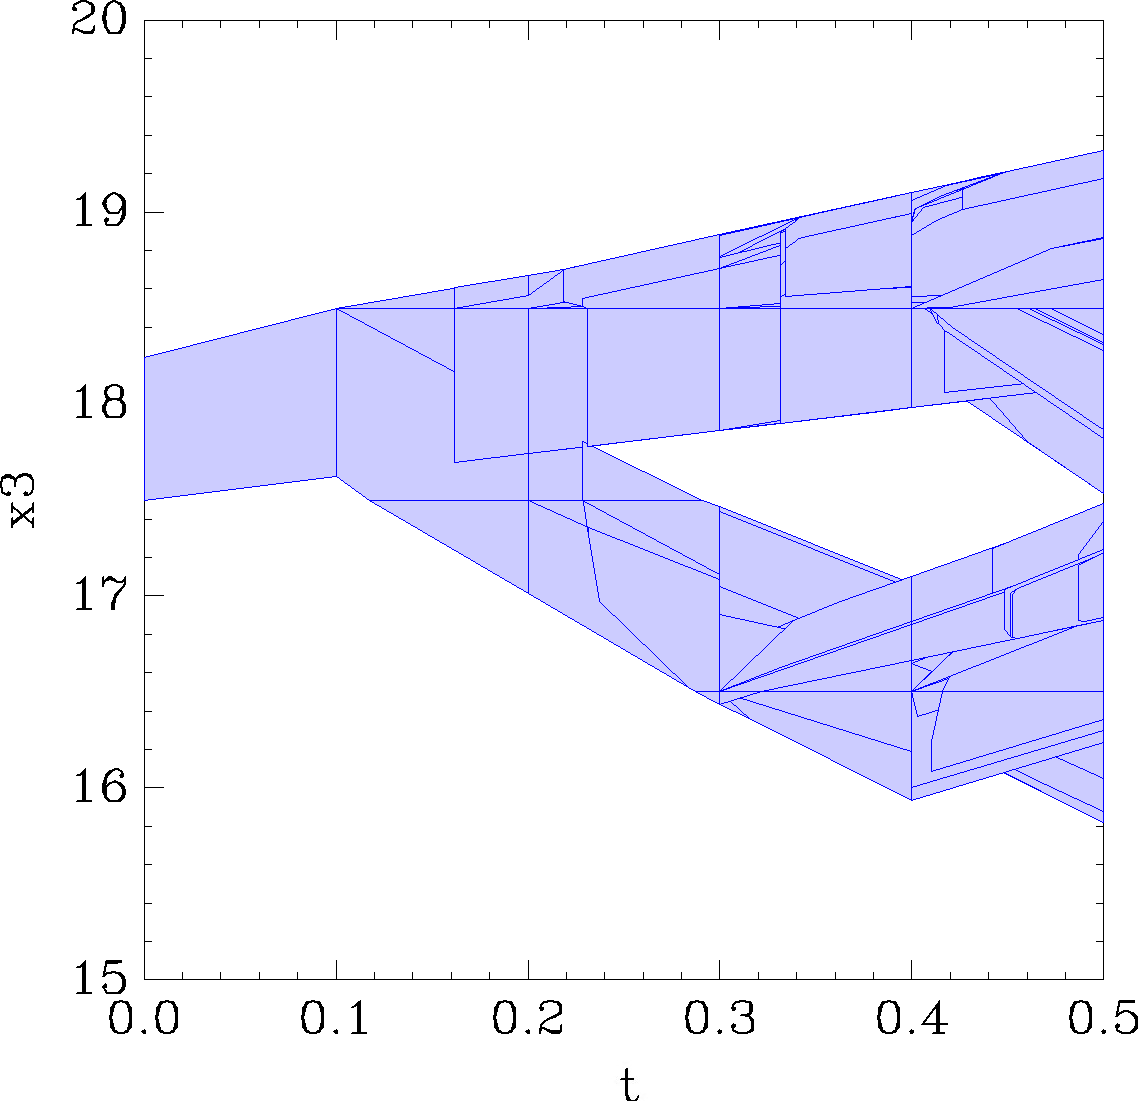
\includegraphics[width=3.5cm]{plot_t_x3}
	\subfigure[Trajectories]{
		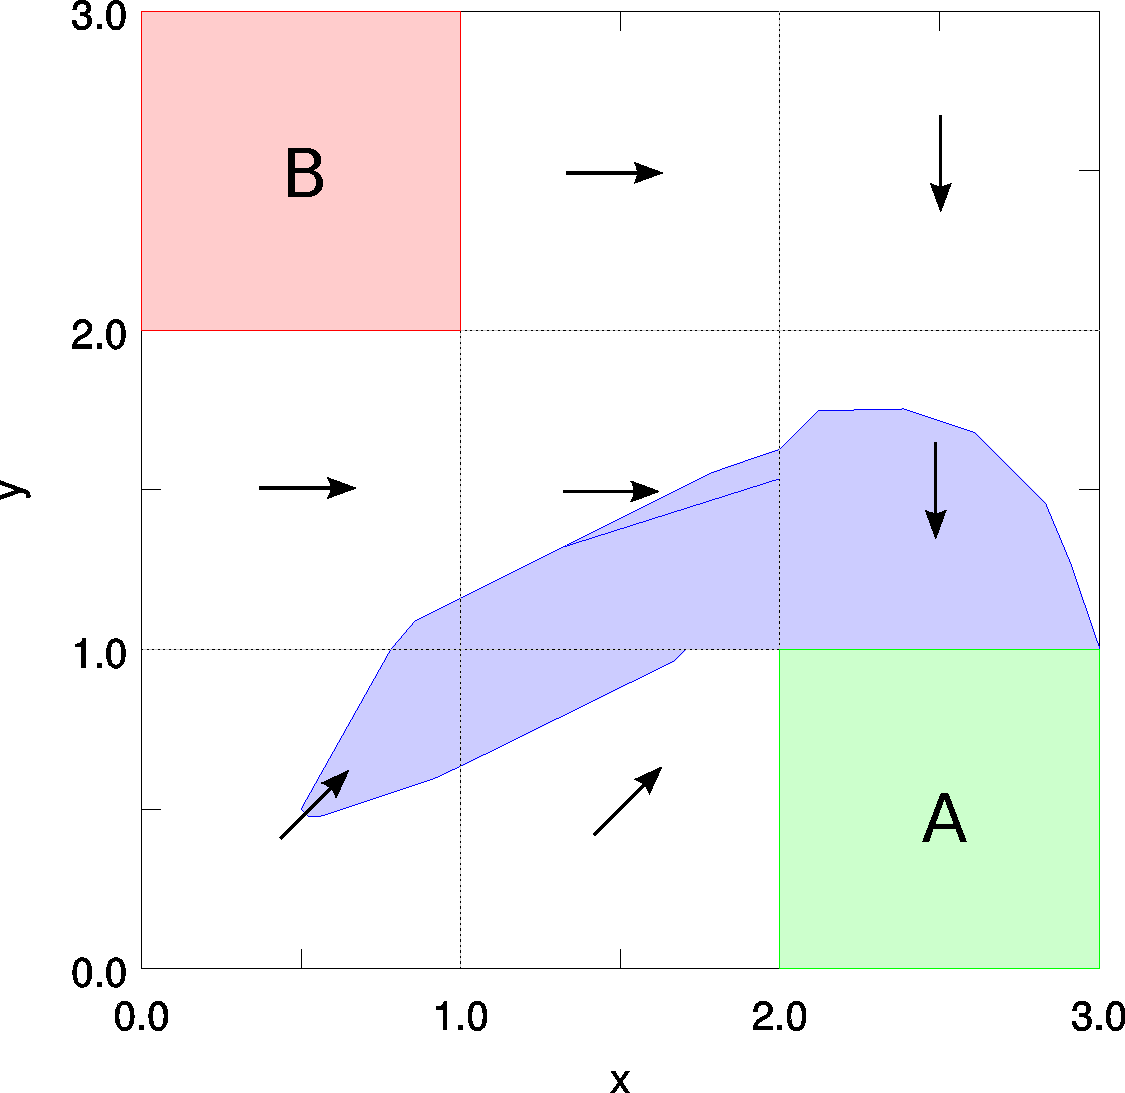
\includegraphics[width=3.6cm]{navigation_map.pdf}
		\label{fig:plot2}
	}
	\subfigure[Behavioral cartography]{
		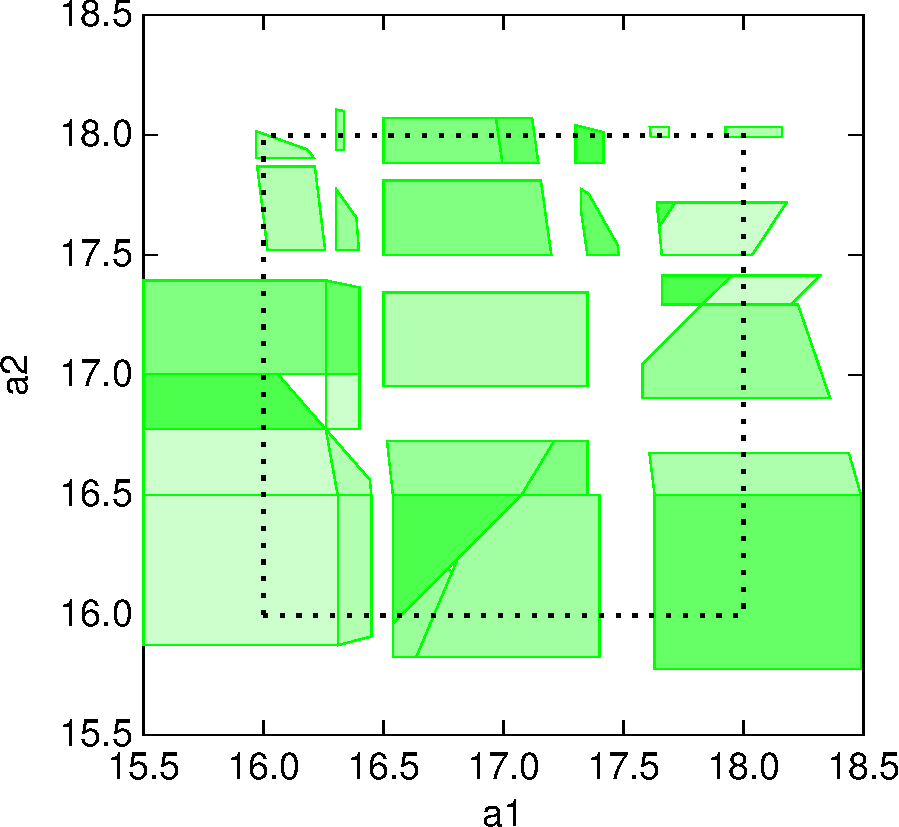
\includegraphics[height=3.6cm]{rhb_cart2.pdf}
		\label{fig:plot3}
	}
%     \label{fig:plot_zone}
%   } 
% 	\caption{a) and b) Set of reachable states c) Behavioral cartography}
	\caption{Examples of graphics output by \hymitator{}}
	\label{fig:plot_rhb}
\end{figure}
%-%-%-%-%-%-%-%-%-%-%-%-%-%-%-%-%-%-%-%-%-%-%-%-%-%-%-%-%-%-%


\hymitator{} can be used for the \emph{parametric verification} of hybrid systems. An application to sampled data hybrid systems has been presented in \cite{FK11}. As a special case, such systems can be parametrized over the initial states. Then, a single run satisfying a desirable reachability property can be generalized to a larger set of initial states. As an example, Figure~\ref{fig:plot1} shows the enlarged reachable states of a single run for the \emph{room   heating benchmark} from~\cite{FI2004}.
This also proves the \emph{robustness} of the system w.r.t.~the tested property. Figure~\ref{fig:plot2} shows an over-approximation of the reachable states for the \emph{navigation benchmark}~\cite{FI2004}, proving that all trajectories will eventually enter the green target zone.

% 
% \begin{figure}[ht]
% \centering
% \subfigure[Caption of subfigure 1]{
% \includegraphics[scale=1]{subfigure1.eps}
% \label{fig:subfig1}
% }
% \subfigure[Caption of subfigure 2]{
% \includegraphics[scale=1]{subfigure2.eps}
% \label{fig:subfig2}
% }
% \subfigure[Caption of subfigure 3]{
% \includegraphics[scale=1]{subfigure3.eps}
% \label{fig:subfig3}
% }
% \label{fig:subfigureExample}
% \caption[Optional caption for list of figures]{Caption of subfigures \subref{fig:subfig1}, \subref{fig:subfig2} and \subref{fig:subfig3}}
% \end{figure}


Another problem that can be addressed using \hymitator{} is \emph{test   coverage}.
In order to ensure the quality of an implementation of a hybrid system, a set of tests is generated which is then applied to the system.
However, since the state space of hybrid systems is infinite in general, it is hard to decide when enough tests have been performed.
Using the inverse method, a tile (dense set of points) around each test point is generated which entails the same discrete behavior.
This means that any point in this tile can be considered covered.
Figure~\ref{fig:plot3} shows the coverage of a parameter rectangle for the room heating benchmark.
% Each colored ``zone'' is a tile generated from one single point; the reference parameter domain is depicted as a dotted rectangle.

% - synthesis schedulability regions (cf [Cimatti-Palopoli-Ramadian08], [Astrium EADS])

\commentaire{experiences ?}

\commentaire{rapport d'etudes de cas a rediger}



%%%%%%%%%%%%%%%%%%%%%%%%%%%%%%%%%%%%%%%%%%%%%%%%%%%%%%%%%%%%
%%%%%%%%%%%%%%%%%%%%%%%%%%%%%%%%%%%%%%%%%%%%%%%%%%%%%%%%%%%%
\section{Related Work}
%%%%%%%%%%%%%%%%%%%%%%%%%%%%%%%%%%%%%%%%%%%%%%%%%%%%%%%%%%%%
%%%%%%%%%%%%%%%%%%%%%%%%%%%%%%%%%%%%%%%%%%%%%%%%%%%%%%%%%%%%

\vspace{-0.1cm}

One of the first powerful model checkers for analyzing hybrid automata is \hytech{}~\cite{hhw97}.
Unfortunately, it can hardly verify even medium sized examples due to exact arithmetics with limited precision and static composition of automata, quickly leading to memory overflows. The tool \phaver{}~\cite{Frehse08} improves on the computation of the reachable states by using efficient over-approximations. Techniques similar to those in \phaver{} have also been implemented in \hymitator{}, with additional algorithmic improvements. The work in \cite{akrs08} presents an analysis on Simulink models which shares similar goals with our approach.

%% \commentaire{to do (citer alur et al)}
% A graphical user interface for the input model is currently under construction, based on a generic platform. \commentaire{utile ?!}

\vspace{-0.1cm}

%%%%%%%%%%%%%%%%%%%%%%%%%%%%%%%%%%%%%%%%%%%%%%%%%%%%%%%%%%%%
%%%%%%%%%%%%%%%%%%%%%%%%%%%%%%%%%%%%%%%%%%%%%%%%%%%%%%%%%%%%
%%%%%%%%%%%%%%%%%%%%%%%%%%%%%%%%%%%%%%%%%%%%%%%%%%%%%%%%%%%%
\bibliographystyle{abbrv} % alpha plain
\bibliography{biblioFM}
%%%%%%%%%%%%%%%%%%%%%%%%%%%%%%%%%%%%%%%%%%%%%%%%%%%%%%%%%%%%
%%%%%%%%%%%%%%%%%%%%%%%%%%%%%%%%%%%%%%%%%%%%%%%%%%%%%%%%%%%%
%%%%%%%%%%%%%%%%%%%%%%%%%%%%%%%%%%%%%%%%%%%%%%%%%%%%%%%%%%%%

% \newpage
% 
% 
% \appendix
% 
% \section*{Appendix}
% 
% \subsection*{Summary of Experiments}
% 
% \commentaire{ajouter un beau tableau avec des contraintes, et un lien vers un rapport d'etudes de cas (+ site Web)}
% 
% \subsection*{Example of Trace Set}
% 
% \commentaire{ajouter un trace set en mode fancy}
% 
% \subsection*{An Example of Model}
% 
% \commentaire{ajouter un modele en entree avec sa representation graphique (pour decrire la syntaxe)}

\end{document}          
